\section{Grundlagen}
\begin{frame}
Hauptbefehle:
\begin{itemize}
%	\item <1->init
%	\note<1>{den Aktuellen Ordner zu einem Git Repository machen}
	\item <2->add
		\note<2>{Dateien/Änderungen zu einem aktuelle commit hinzufügen}
	\item <3->commit
		\note<3>[item]{Commits sind eingetragene Änderungen}
		\note<3>[item]{Diese Einträge sollten immer einen Titel haben der die Änderungen beschreiben}
		\note<3>[item]{Dabei sollte man eine Struktur einhalten, mehr dazu später.}
		\note<3>[item]{Vorsicht: Nach dem eine Änderung commited wurde ist sie noch nicht im Master Projekt zu finden. }
		\note<3>[item]{Dafür müssen die Änderungen...(push)}
	\item <4->push
		\note<4>[item]{Push leitet Vorgang ein, temporären Änderungen einzutragen}
	\item <5->pull
		\note<5>[item]{Pull wird zum kopieren des aktuellen Zustandes des Masterprojektes benutzt}
		\note<5>[item]{Alle gepushden Änderungen werden kopiert}
	\item <6->branch
		\note[item]<6>{Erstellung eines parallelen Stranges eines Projektes}
		\note[item]<6>{Master Branch besteht immer}
		\note[item]<6>{Man kann auf beiden Branches normal weiter arbeiten}
		\note[item]<6>{Bsp.: longtime Support alter Software und neue Version}
	\item <7->merge
		\note[item]<7>{Zusammenführen von branches}
		\note<7>[item]{Kann automatisch passieren}
		\note<7>[item]{Gleiche Passagen müssen per Hand gemacht werden}
\end{itemize}
\end{frame}
\begin{frame}
	
\includegraphics[scale=0.3]{Bilder/git_graph1}
	\note{Beispiel eines git Projektverlaufes}
\end{frame}
\begin{frame}
	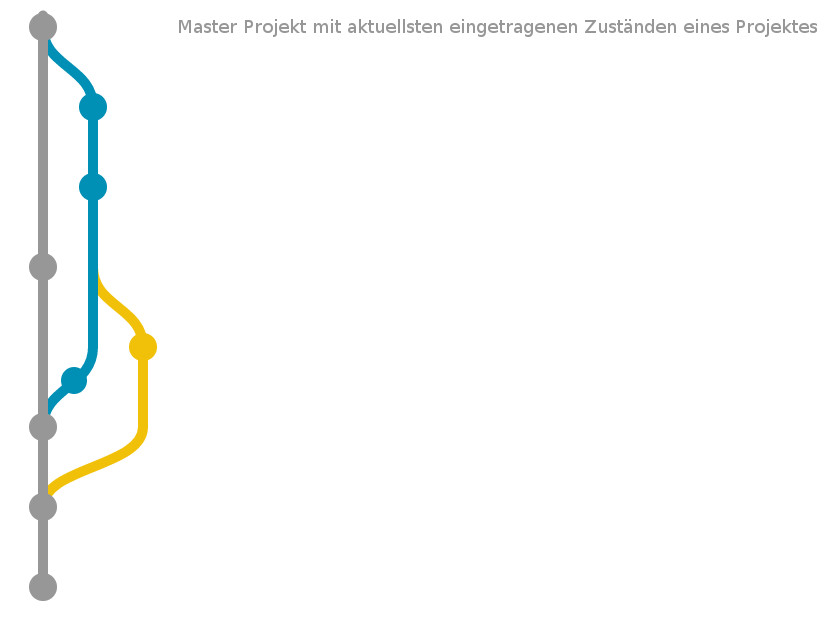
\includegraphics[scale=0.3]{Bilder/git_graph2}
	\note{Graue Linie: Master Projekt mit aktuellsten Änderungen. Alles geht zurück auf das Master Projekt. Es existiert immer nur ein Projekt mit dem interagiert wird.}
\end{frame}
\begin{frame}
	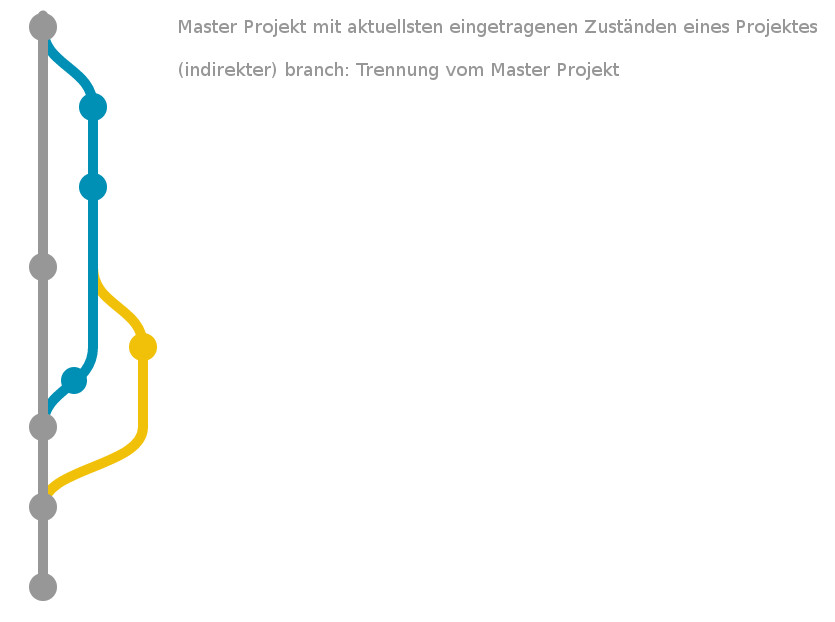
\includegraphics[scale=0.3]{Bilder/git_graph3}
	\note{Bei einer Änderung wird ein indirekter Branch einer Projektes erstellt, wie zum Beispiel bei einem...(commit)}
\end{frame}
\begin{frame}
	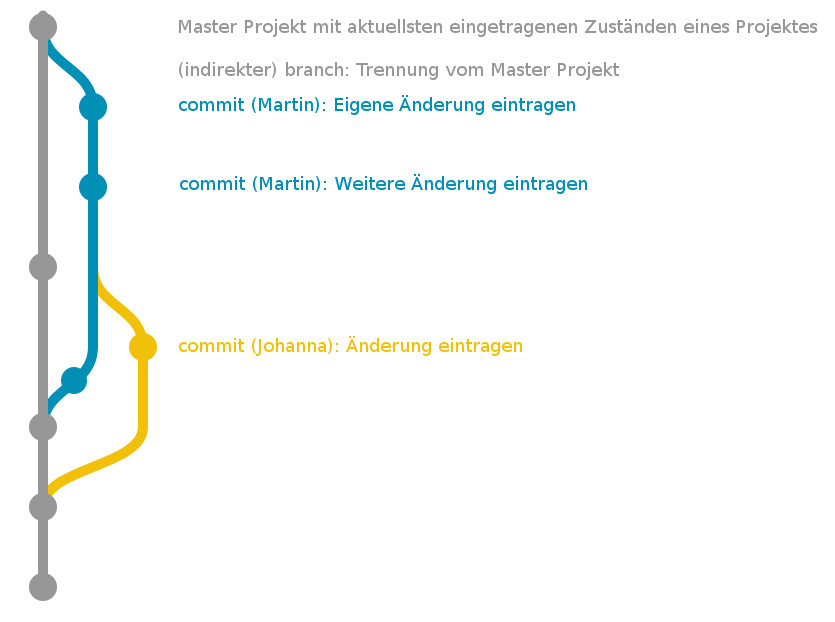
\includegraphics[scale=0.3]{Bilder/git_graph4}
\end{frame}
\begin{frame}
	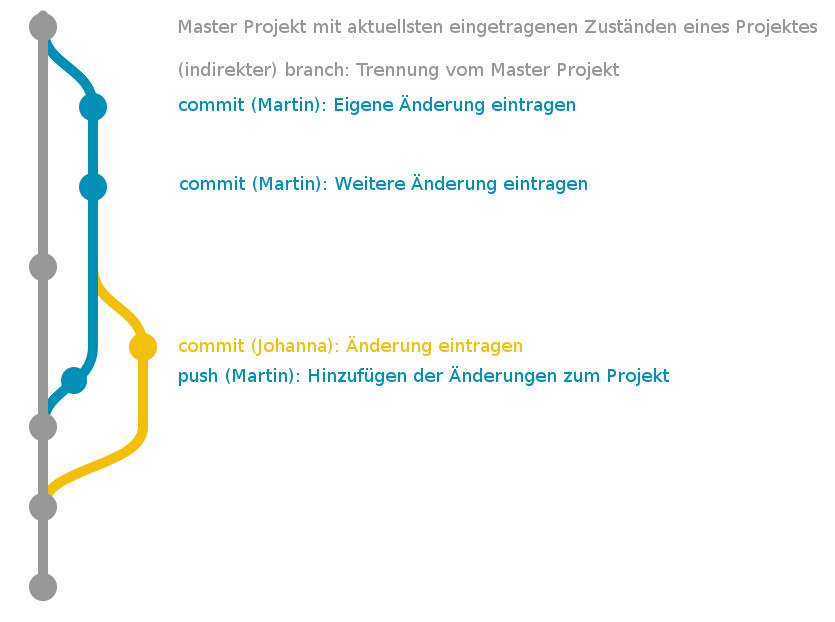
\includegraphics[scale=0.3]{Bilder/git_graph5}
\end{frame}
\begin{frame}
	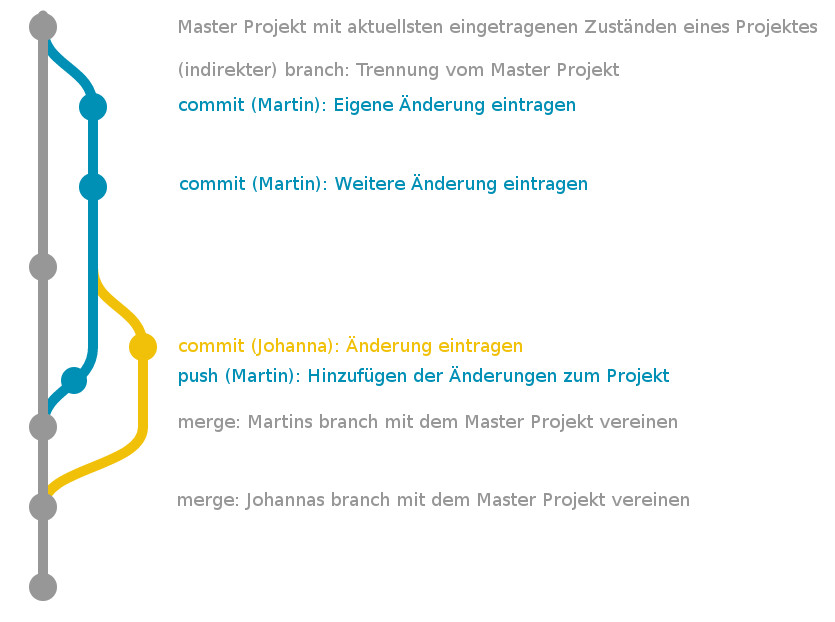
\includegraphics[scale=0.3]{Bilder/git_graph6}
	\note{Beim zusammenführen der Dateien zum Master Projekt wird ein merge gemacht, damit sind nun die Änderungen in das Master Projekt eingetragen worden}
\end{frame}
\subsection{Details}
\begin{frame}
Hier noch ein paar Details.
\end{frame}